%\documentclass{beamer}
\documentclass[aspectratio=141]{beamer}
\usepackage[utf8]{inputenc}
\usepackage[T1]{fontenc}
\usepackage{mathtools}
\usepackage{graphicx}
\usepackage{caption}
\usepackage{tikz}
\usepackage{pgfplots}
\usepackage{amsmath, amssymb, amsthm}
\usepackage{multimedia}
\usepackage{bbm}
\usepackage{mathrsfs}
\DeclareMathAlphabet{\mathdutchcal}{U}{dutchcal}{m}{n}
\SetMathAlphabet{\mathdutchcal}{bold}{U}{dutchcal}{b}{n}
\DeclareMathAlphabet{\mathdutchbcal}{U}{dutchcal}{b}{n}
\usepackage{aligned-overset}
\usepackage{color}
\usepackage{comment}

%\usepackage[backend=bibtex,style=numeric,sorting=nyt]{biblatex}
%\addbibresource{bibliografia.bib}
\captionsetup{labelformat=empty,labelsep=none}
%\useoutertheme{miniframes}
%\setbeamercolor{section in head/foot}{bg=blue, fg=white}
%\setbeamercolor{subsection in head/foot}{bg=blue!50, fg=white}
\usepackage[
backend=bibtex,
style=draft,
sorting=nyt
]{biblatex}
\addbibresource{bibliografiapresentazione.bib}
\newcommand\setItemnumber[1]{\setcounter{enumi}{\numexpr#1-1\relax}}

\newcommand{\R}{\mathbb{R}} %scorciatoia per R reali
\newcommand{\N}{\mathbb{N}} %scorciatoia per N naturali
\newcommand{\Q}{\mathbb{Q}} %scorciatioia per Q razionali
\newcommand{\V}{\mathcal{V}} %STFT
\newcommand{\F}{\mathscr{F}} %Fourier transform
\newcommand{\Fock}{\mathcal{F}} %Fock space
\newcommand{\C}{\mathbb{C}} %Complex numbers
\newcommand{\B}{\mathscr{B}} %Bounded linear operators
\newcommand{\Barg}{\mathcal{B}} %Bargmann transform
\renewcommand{\L}{\mathscr{L}} %sesquilinear form localization operator
\newcommand{\dxdo}{\,dx\,d\omega}
\newcommand{\notazione}{\underline{\textbf{Remark Notazionale}}}
\newcommand{\Log}{\ensuremath{\mathrm{Log}_-}}
\newcommand{\finire}{\fbox{\LARGE DA FINIRE}}
\newcommand{\pdfrac}[2]{\dfrac{\partial #1}{\partial #2}}
\newcommand{\pfrac}[2]{\frac{\partial #1}{\partial #2}}
\DeclareMathOperator*{\esssup}{ess\,sup}
\newcommand{\emptyline}{\phantom{ }\\}

\title[Recent results on the norm of localization operators]{Recent results on the norm of localization operators}
\date[ISPN ’80]{Laurea Magistrale in Ingegneria Matematica}
\author[F. Riccardi]{Federico Riccardi}

\usetheme{DE}

\setbeamertemplate{footline}[my footline]

\begin{document}
	


\begin{frame}
\titlepage
\end{frame}

%\setbeamertemplate{footline}{}

\begin{section}{Introduzione}
	
	\begin{frame}
		\frametitle{Introduzione}
		\begin{itemize}
			\item \textbf{Problema}: elaborare un segnale, ad esempio una traccia audio, un'immagine, una misurazione di un sensore, ecc.;\\
			\pause
			\emptyline
			\item \textbf{Motivazioni}: analizzare il segnale ed estrarne informazioni rilevanti, separare delle componenti, filtrare elementi non desiderati;\\
			\pause
			\emptyline
			\item \textbf{Come fare}: trasformate, ad esempio la trasformata di Fourier $\F$, trasformate tempo-frequenza, come la short-time Fourier transform, filtri, operatori di localizzazione.
		\end{itemize}
	\end{frame}

	\begin{frame}
		\frametitle{Introduzione}
		\framesubtitle{Principi di indeterminazione}
		L'obiettivo di localizzare un segnale si scontra con un limite fondamentale, ovvero i \emph{principi di indeterminazione}. Esistono numerosi principi di indeterminazione, ognuno espressione del seguente concetto:
		\begin{center}
			\emph{una funzione non può essere troppo concentrata sia in tempo che in frequenza}.
		\end{center}
		\begin{center}
			\begin{figure}
				\scalebox{1}{
				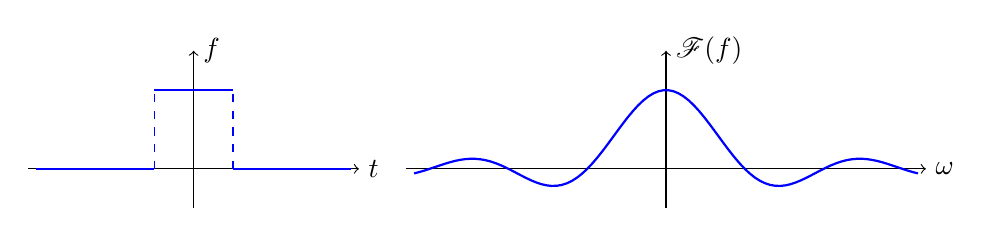
\begin{tikzpicture}
					%\draw[very thin,color=gray] (-6,-2.5) grid (6,2.5);
					\coordinate (L) at (-3,0);
					\coordinate (R) at (3,0);
					%\draw[->] (-6,0) --  (6,0);
					%\draw[->] (0, -2.5) -- (0, 2.5);
					\draw[->, shift={(L)}] (-2.1, 0) -- (2.1, 0) node[right]{$t$};
					\draw[->, shift={(L)}] (0, -0.5) -- (0, 1.5) node[right]{$f$};
					\draw[thick, blue, shift={(L)}] plot[domain=-2:-0.5] (\x,0);
					\draw[dashed, blue, shift={(L)}] (-0.5, 0) -- (-0.5, 1);
					\draw[thick, blue, shift={(L)}] plot[domain=-0.5:0.5] (\x,1);
					\draw[dashed, blue, shift={(L)}] (0.5, 0) -- (0.5, 1);
					\draw[thick, blue, shift={(L)}] plot[domain=0.5:2] (\x,0);
					
					\draw[->, shift={(R)}] (-3.3, 0) -- (3.3, 0) node[right]{$\omega$};
					\draw[->, shift={(R)}] (0, -0.5) -- (0, 1.5) node[right]{$\F(f)$};
					\draw[thick, blue, shift={(R)}] plot[domain=-3.2:3.2, samples=100] (\x, {sin(3.14*deg(\x))/(3.14*\x)});
				\end{tikzpicture}}
			\caption{Esempio di funzione ben concentrata in tempo con trasformata poco concentrata in frequenza.}
			\end{figure}
		\end{center}
	\end{frame}

	\begin{frame}
		\frametitle{Introduzione}
		\framesubtitle{Esempio: principio di indeterminazione di Heisenberg}
		\begin{myblock}[Principio di indeterminazione di Heisenberg]
			Sia $f \in L^2(\R)$ con $\|f\|_2 = 1$ e siano $a,b \in \R$. Allora:
			\begin{equation}
				\left(\int_{\R} (t-a)^2 |f(t)|^2 \, dt\right)^{1/2} \left(\int_{\R} (\omega-b)^2 |\F f(\omega)|^2 \, d\omega	\right)^{1/2} \geq \dfrac{1}{4 \pi}.
			\end{equation}
			Le funzioni che raggiungono l'uguaglianza sono solo le gaussiane.
		\end{myblock}
		\textbf{Interpretazione}: i due integrali si possono vedere come misure della concentrazione di $f$ e $\F f$ vicino ai punti $a$ e $b$, rispettivamente. Se una delle concentrazioni è ``piccola'', l'altra deve essere ``grande''.\\
	\end{frame}
	
\end{section}

\begin{section}{Short-time Fourier transform}
	\begin{frame}
		\frametitle{Short-time Fourier transform}
		\framesubtitle{Definizione}
		La \emph{short-time Fourier transform}, in breve \emph{STFT}, è una trasformata tempo-frequenza. Prima di definirla, dobbiamo introdurre gli operatori di traslazione e modulazione. Dati $x, \omega \in \R$ abbiamo:
		\begin{equation*}
			T_x f(t) = f(t-x), \quad M_{\omega} f(t) = e^{2 \pi i \omega t} f(t).
		\end{equation*}
		\pause
		\begin{myblock}[Short-time Fourier transfrom]
			La short-time Fourier transform di una funzione $f \in L^2(\R)$ rispetto alla finestra $\phi \in L^2(\R)$ è data da:
			\begin{equation*}
				\V_{\phi} f(x, \omega) = \langle f, M_{\omega} T_x \phi \rangle = \int_{\R} f(t) \overline{\phi(t-x)} e^{-2 \pi i \omega t} \, dt.
			\end{equation*}
		\end{myblock}
	\end{frame}

	\begin{frame}
		\frametitle{Short-time Fourier transform}
		\framesubtitle{Finestra gaussiana}
		\begin{center}
			\begin{figure}
				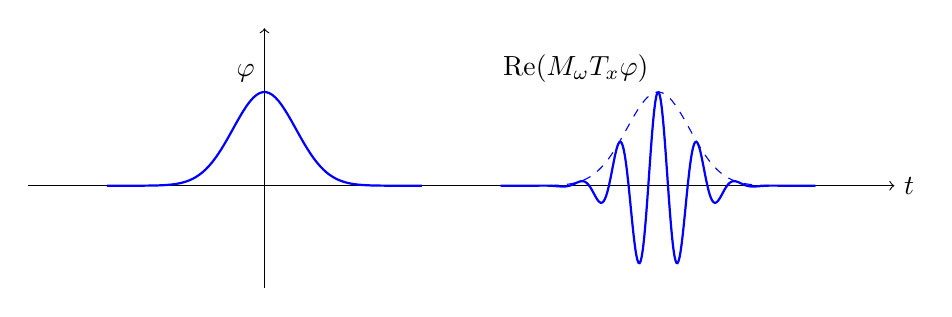
\begin{tikzpicture}
					\coordinate (T) at (-3,0);
					\coordinate (S) at (2,0);
					\draw[->, shift={(T)}] (0,-1.3) -- (0,2);
					\draw[->] (-6, 0) -- (5, 0) node[right]{$t$};
					%\draw (-6,-2) grid (6,2);
					\draw[thick, blue, shift={(T)}] plot[domain=-2:2, samples=100] (\x, {1.19*exp(-3.14*(\x)^2)});
					\draw[shift={(T)}] (0,1.19) node[above left]{$\varphi$};
					\draw[dashed, blue, shift={(S)}] plot[domain=-2:2, samples=100] (\x, {1.19*exp(-3.14*(\x)^2)});
					\draw[shift={(S)}] (0,1.19) node[above left]{$\mathrm{Re}(M_{\omega} T_x\varphi)$};
					\draw[thick, blue, shift={(S)}] plot[domain=-2:2, samples=300] (\x, {1.19*exp(-3.14*(\x)^2)*cos(4*3.14*deg(\x))});					
				\end{tikzpicture}
			\end{figure}
		\end{center}
		Per avere una buona risoluzione è necessario scegliere una finestra ben localizzata sia in tempo che in frequenza. Una scelta ottimale è quindi una finestra gaussiana normalizzata in $L^2$
		\begin{equation*}
			\varphi(t) = 2^{1/4} e^{-\pi t^2}.
		\end{equation*}
		
	\end{frame}
\end{section}

\begin{section}{Operatori di localizzazione in tempo-frequenza}
	
	\begin{frame}
		\frametitle{Operatori di localizzazione in tempo-frequenza}
		\framesubtitle{Definizione}
		Con la particolare scelta di finestra gaussiana normalizzata l'operatore $\V_{\varphi} : L^2(\R) \rightarrow L^2(\R^2)$ diventa un'isometria e vale la seguente formula di inversione:
		\begin{equation*}
			\V_{\varphi}^* \V_{\varphi} = I_{L^2(\R)}.
		\end{equation*}
		\pause
		Questo suggerisce come definire un operatore di localizzazione:
		\begin{equation*}
			f \in L^2(\R) \pause \mapsto \V_{\varphi} f \in L^2(\R^2) \pause \mapsto F \V_{\varphi} f \in L^2(\R^2) \pause \mapsto \V_{\varphi}^* F \V_{\varphi} f \in L^2(\R)
		\end{equation*}
		\onslide<5-> \begin{myblock}[Operatore di localizzazione in tempo-frequenza - Daubechies 1988]
			Data una finestra $F: \R^2 \rightarrow \C$, l'operatore di localizzazione in tempo-frequenza con finestra $\varphi$ e peso $F$ è definito da
			\begin{equation*}
				L_{F,\varphi} \coloneqq \V_{\varphi}^* F \V_{\varphi} : L^2(\R) \rightarrow L^2(\R).
			\end{equation*}
		\end{myblock}
	\end{frame}

	\begin{frame}
		\frametitle{Operatori di localizzazione in tempo-frequenza}
		\framesubtitle{Proprietà}
		Le proprietà di $L_{F,\varphi}$ dipendono dalle caratteristiche della funzione peso $F$:
		\begin{itemize}
			\item se $F \in L^p (\R^2)$ con $p \in [1,+\infty]$ allora $L_{F,\varphi}$ è limitato e $\|L_{F,\varphi}\| \leq \|F\|_p$; \pause
			\item se $F \in L^p (\R^2)$ con $p \in [1,+\infty)$ allora $L_{F,\varphi}$ è compatto;\pause
			\item se $F \in L^2(\R^2)$ allora $L_{F,\varphi}$ è un operatore integrale di Hilbert-Schmidt e la sua norma di Hilbert-Schmidt è minore o uguale di $\|F\|_1$;\pause
			\item se $F \in L^1(\R^2)$ è un operatore di classe traccia;\pause
			\item se $F$ è radialmente simmetrica, ovvero $F(x,\omega) = \mathdutchcal{F}(r^2)$ con $r^2 = x^2 + \omega^2$, le autofunzioni di $L_{F,\varphi}$ sono le funzioni di Hermite e i corrispondenti autovalori sono dati da
			\begin{equation*}
				\lambda_k = \dfrac{1}{k!} \int_0^{+\infty} \mathdutchcal{F}\left(\dfrac{s}{\pi}\right) s^k e^{-s} \, ds.
			\end{equation*}
		\end{itemize}
	\end{frame}
\end{section}

\begin{section}{Stime norma operatori di localizzazione}
	
	\begin{frame}
		\frametitle{Stime sulla norma di operatori di localizzazione}
		\framesubtitle{Disuguaglianza di Lieb}
		Oltre alle proprietà appena elencate, è interessante studiare il problema di trovare delle stime sharp per la norma degli operatori di localizzazione.
		\pause
		\begin{myblock}[Disuguaglianza di Lieb - Lieb 1978]
			Sia $p \in (1,+\infty)$. Allora, per ogni $F \in L^p(\R^2)$ vale
			\begin{equation}\label{stima Lieb}
				\|L_{F,\varphi}\| \leq \left(\dfrac{p-1}{p}\right)^{\frac{p-1}{p}} \|F\|_p,
			\end{equation}
			con uguaglianza se e solo se $F$ è una gaussiana, eventualmente traslata e modulata.
		\end{myblock}
	\end{frame}

	\begin{frame}
		\frametitle{Stime sulla norma di operatori di localizzazione}
		\framesubtitle{Disuguaglianza di Faber-Krahn per la STFT}
		Alcuni risultati su questo problema sono stati ottenuti solo recentemente.
		\begin{myblock}[Disuguaglianza di Faber-Krahn per la STFT - Nicola e Tilli 2022]
			Sia $\Omega \subset \R^2$ un insieme misurabile di misura finita. Allora, indicando con $L_{\Omega, \varphi}$ l'operatore di localizzazione con peso pari alla funzione indicatrice di $\Omega$, si ha:
			\begin{equation*}
				\|L_{\Omega, \varphi}\| \leq 1 - e^{- |\Omega|},
			\end{equation*}
			con uguaglianza se e solo se $\Omega$ è una palla.
		\end{myblock}
	\end{frame}
	
	\begin{comment}
	\begin{frame}
		\frametitle{Stime sulla norma di operatori di localizzazione}
		\framesubtitle{Disuguaglianza di Faber-Krahn per la STFT}
		Recentemente, il seguente risultato è stato ottenuto in [Nicola e Tilli 2022].
		\begin{myblock}[Disuguaglianza di Faber-Krahn per la STFT]
			Dato $\Omega \subset \R^2$ misurabile di misura finita si ha
			\begin{equation}\label{faber-krahn stft}
				\int_{\Omega} |\V_{\varphi} f (x, \omega)|^2 \, dx \, d\omega \leq ( 1 - e^{-|\Omega|}) \int_{\R^2} |\V_{\varphi} f (x, \omega)|^2\,dx\,d\omega,
			\end{equation}
			con uguaglianza se e solo se $\Omega$ è una palla di centro $(x_0, \omega_0) \in \R^2$ e $f$ è una gaussiana traslata e modulata, ovvero $f = c M_{\omega_0} T_{x_0} \varphi$ con $c \in \C \setminus \{0\}$.
		\end{myblock}
	\end{frame}

	
	\begin{frame}
		\frametitle{Risultati recenti}
		\framesubtitle{Disuguaglianza di Faber-Krahn per la STFT}
		Questo risultato può essere riformulato in termini di norma di  operatori di localizzazione con funzione indicatrice come peso. Infatti:
		\begin{equation*}
			\int_{\Omega} |\V_{\varphi} f (x, \omega)|^2 \, dx \, d\omega = \langle \chi_{\Omega} \V_{\varphi} f, \V_{\varphi} f \rangle = \langle \V_{\varphi}^* \chi_{\Omega} \V_{\varphi} f, f \rangle = \langle L_{\Omega, \varphi} f, f \rangle.
		\end{equation*}
		\pause
		Poiché $\V_{\varphi}$ è un'isometria, da \eqref{faber-krahn stft} otteniamo:
		\begin{equation*}
			\langle L_{\Omega, \varphi} f, f \rangle \leq (1-e^{-|\Omega|}) \|f\|_2^2.
		\end{equation*}
		Prendendo l'estremo superiore fra tutte le $f \in L^2(\R)$ normalizzate, poiché $L_{\Omega, \varphi}$ è compatto e autoaggiunto, si ottiene
		\begin{equation*}
			\|L_{\Omega, \varphi} \| \leq 1 - e^{-|\Omega|},
		\end{equation*}
		con uguaglianza se e solo se $\Omega$ è una palla.
	\end{frame}
	
	\begin{frame}
		\frametitle{Risultati recenti}
		\framesubtitle{Stime ottimali sulla norma di $L_{F,\varphi}$: vincoli $L^p$ e $L^{\infty}$}
		Se immaginiamo quindi di fissare un limite $s$ alla misura di $\Omega$, quanto ottenuto ci dice che se $|\Omega| \leq s$ allora $\|L_{\Omega, \varphi}\| \leq 1 - e^{-s}$.\\
		\pause
		Anziché considerare solo funzioni indicatrici, si potrebbero prendere funzioni peso generiche $F$ e tradurre il vincolo $|\Omega| \leq s$ in un vincolo sulla norma di $F$ in qualche spazio di Lebesgue.
		\pause
		In [Nicola e Tilli 2023] è stato considerato il seguente problema:
		\begin{center}
			trovare $C>0$ tale che $\|L_{F,\varphi}\| \leq C$ per ogni $F$ che soddisfa\\
			$\|F\|_{\infty} \leq A$ e $\|F\|_{p} \leq B$,			
		\end{center}
		dove $p \in [1,+\infty)$, $A \in (0, +\infty]$ e $B \in (0, +\infty)$.
	\end{frame}
	\end{comment}

	\begin{frame}
		\frametitle{Stime sulla norma di operatori di localizzazione}
		\framesubtitle{Risultati recenti: $F \in L^p \cap L^{\infty}$}
		Grazie al risultato precedente è possibile trattare il caso in cui il peso $F$ sia generico e non solo una funzione indicatrice. In questa direzione, in [Nicola e Tilli 2023] è stato studiato il seguente problema:
		\begin{center}
			trovare $C>0$ tale che $\|L_{F,\varphi}\| \leq C$ per ogni $F$ che soddisfa\\
			$\|F\|_{\infty} \leq A$ e $\|F\|_{p} \leq B$,			
		\end{center}
		dove $p \in [1,+\infty)$, $A \in (0, +\infty]$ e $B \in (0, +\infty)$ (con la condizione aggiuntiva $A<+\infty$ se $p=1$). Presentiamo il risultato nel caso $p>1$.
	\end{frame}

	\begin{frame}
		\frametitle{Stime sulla norma di operatori di localizzazione}
		\framesubtitle{Risultati recenti: $F \in L^p \cap L^{\infty}$}
		\begin{myblock}[Teorema - Nicola e Tilli 2023]
			Sia $p \in (1, +\infty)$ e sia $F \in L^p(\R^2) \cap L^{\infty}(\R^2)$. Allora:
			\begin{enumerate}
				\item se $\|F\|_p / \|F\|_{\infty}  \leq (p-1)/p$ la stima \eqref{stima Lieb} resta ottimale;
				\pause
				\item se $\|F\|_p / \|F\|_{\infty} > (p-1)/p$ allora
				\begin{equation*}
					\|L_{F,\varphi}\| \leq \|F\|_{\infty} \left(1 - \dfrac{e^{(p-1)/p - (\|F\|_p / \|F\|_{\infty})^p}}{p}\right),
				\end{equation*}
				con uguaglianza se e solo se $F$ è (a meno di traslazioni e modulazioni) una \emph{gaussiana troncata in alto}, ovvero della forma
				\begin{equation*}
					F(x,\omega) = \min \{\lambda e^{-\frac{\pi}{p-1}(x^2 + \omega^2)}, A\}.
				\end{equation*}
				per qualche $\lambda > A$.
			\end{enumerate}
		\end{myblock}
	\end{frame}


	\begin{frame}
		\frametitle{Stime sulla norma di operatori di localizzazione}
		\framesubtitle{Risultati recenti: $F \in L^p \cap L^q$}
		Nella mia tesi ho considerato l'analogo problema con due vincoli di tipo $L^p$:
		\begin{center}
			trovare $C>0$ tale che $\|L_{F,\varphi}\| \leq C$ per ogni $F$ che soddisfa\\
			$\|F\|_{p} \leq A$ e $\|F\|_{q} \leq B$,			
		\end{center}
		dove $p, q \in (1,+\infty)$, $A,B \in (0, +\infty)$.
	\end{frame}

	\begin{frame}
		\frametitle{Stime sulla norma di operatori di localizzazione}
		\framesubtitle{Risultati recenti: $F \in L^p \cap L^q$}
		\begin{myblock}[Teorema]
			Siano $p,q \in (1,+\infty)$ e sia $F \in L^p(\R^2) \cap L^q(\R^2)$. Allora esistono due costanti $c_1 < c_2$, che dipendono solo da $p$ e $q$, tali che:
			\begin{enumerate}
				\item se $\|F\|_q / \|F\|_p \leq c_1$ o se $\|F\|_q / \|F\|_p \geq c_2$, la stima \eqref{stima Lieb} resta ottimale, con $p$ e $q$ rispettivamente.
			\end{enumerate}
		\end{myblock}
	\end{frame}
	
	\begin{frame}
		\frametitle{Stime sulla norma di operatori di localizzazione}
		\framesubtitle{Risultati recenti: $F \in L^p \cap L^q$}
		\begin{myblock}[Teorema]
			{\small Siano $p,q \in (1,+\infty)$ e sia $F \in L^p(\R^2) \cap L^q(\R^2)$. Allora esistono due costanti $c_1 < c_2$, che dipendono solo da $p$ e $q$, tali che:
			\begin{enumerate}
				\setItemnumber{2}
				\item se $c_1 < \|F\|_q / \|F\|_p < c_2$ allora
				\begin{equation}\label{norm limitation generic case}
					\|L_{F,\varphi}\| \leq T - \lambda_1 T^p/p - \lambda_2 T^q/q,
				\end{equation}
				dove $\lambda_1, \lambda_2 > 0$ sono univocamente determinati da
				\begin{equation*}
					p \int_{0}^{+\infty} t^{p-1} u(t) \, dt = A^p, \quad q \int_{0}^{+\infty} t^{q-1} u(t) \, dt = B^q,
				\end{equation*}
				con $u(t) = \max\{-\log(\lambda_1 t^{p-1} + \lambda_2 t^{q-1}), 0\}$ e $T>0$ tale che $\lambda_1 T^{p-1} + \lambda_2 T^{q-1}=1$. Infine, l'uguaglianza in \eqref{norm limitation generic case} si ha se e solo se $F$ è (a meno di traslazioni e modulazioni) radialmente simmetrica e ha $u$ come funzione di distribuzione.
			\end{enumerate}}
		\end{myblock}
	\end{frame}

	\begin{frame}
		\frametitle{Stime sulla norma di operatori di localizzazione}
		\framesubtitle{Idea della dimostrazione nel secondo regime}
		\begin{itemize}
			\item Il primo passo viene suggerito da un teorema presente in [Nicola e Tilli 2023].
			\begin{myblock}[Teorema]
				Data $F \in L^p(\R^2)$ con $p \in [1,+\infty)$ e indicando con $\mu(t) = |\{|F|>t\}|$ la funzione di distribuzione di $|F|$, si ha
				\begin{equation*}
					\|L_{F,\varphi}\| \leq \int_{0}^{+\infty} (1-e^{-\mu(t)}) \, dt,
				\end{equation*}
				con uguaglianza se e solo se $F$ è (a meno di traslazioni) radialmente simmetrica.
			\end{myblock}
			Questo ci indica che è necessario trovare stime sharp per il membro destro.
		\end{itemize}
	\end{frame}

	\begin{frame}
		\frametitle{Stime sulla norma di operatori di localizzazione}
		\framesubtitle{Idea della dimostrazione nel secondo regime}
		\begin{itemize}
			\item Il problema variazionale per la funzione di distribuzione, dopo un'opportuna traduzione dei vincoli di integrabilità, è il seguente:
			\begin{equation*}
				\sup_{v \in \mathcal{C}} \int_0^{+\infty} (1-e^{-v(t)}) \, dt
			\end{equation*}
			dove $\mathcal{C}$ è l'insieme dell funzioni  $v : (0, +\infty) \rightarrow [0, +\infty)$ decrescenti e che soddisfano i vincoli
			\begin{equation*}
				p\int_{0}^{+\infty} t^{p-1} v(t) \, dt \leq A^p,\quad q\int_{0}^{+\infty} t^{q-1} v(t) \, dt \leq B^q .
			\end{equation*} 
		\end{itemize}
	\end{frame}

	\begin{frame}
		\frametitle{Stime sulla norma di operatori di localizzazione}
		\framesubtitle{Idea della dimostrazione nel secondo regime}
		\begin{itemize}
			\item Una volta dimostrata l'esistenza di soluzioni per il problema variazionale, si dimostra che le funzioni estremali sono della forma
			\begin{equation*}\label{expression u}
				u(t) = \begin{cases}
					-\log\left(\lambda_1 t^{p-1} + \lambda_2 t^{q-1}\right) & t \in (0,M)\\
					0 & t \in (M,+\infty)
				\end{cases}
			\end{equation*}
			per qualche $M>0$ e $\lambda_1, \lambda_2 \in \R$.
		\end{itemize}
		\begin{columns}[onlytextwidth,T]
			\begin{column}{.45\linewidth}
				\begin{figure}
					\begin{tikzpicture}
						\coordinate (T) at (-3,0);
						\draw[->, shift={(T)}] (0,-0.1) -- (0,3) node[right]{$u(t)$};
						\draw[->, shift={(T)}] (-0.1, 0) -- (3, 0) node[right]{$t$};
						\draw[densely dashed, blue, shift={(T)}] (1, 0.41369, 0) -- (1, 0);
						\draw[thick, blue, shift={(T)}] plot[domain=0.02:1, samples=100] (\x, {-ln(0.5144*(\x)^0.5 + 0.1468*(\x)^19)});
						\draw[thick, blue, shift={(T)}] (1,0) -- (2.9,0);
						\draw[shift={(T)}] (1,0) + (0,2pt) -- (1,0) + (0, -2pt) -- (1,0) + (0, -2pt) node[below] {\small $M$};
					\end{tikzpicture}
				\end{figure}
			\end{column}
			\begin{column}{.45\linewidth}
				\emptyline
				\emptyline
				\emptyline
				\emptyline
				\begin{flushleft}
					\hspace{-1cm}Esempio di funzione estremale.
				\end{flushleft}				
			\end{column}
		\end{columns}
		\begin{center}
			
		\end{center}
	\end{frame}

	\begin{frame}
		\frametitle{Stime sulla norma di operatori di localizzazione}
		\framesubtitle{Idea della dimostrazione nel secondo regime}
		\begin{itemize}
			\item Gli ultimi step prevedono di dimostrare che gli estremali sono continui e che devono raggiungere l'uguaglianza nei vincoli. Questo permette poi di dimostrare che $\lambda_1, \lambda_2$ sono entrambi positivi e univocamente determinati.
			\pause
			\item Una volta determinata la funzione di distribuzione $u$ ottimale, è semplice ricostruire $F$ tramite riarrangiamento.
		\end{itemize}
	\end{frame}

	\begin{comment}
	\begin{frame}
		\frametitle{Stime sulla norma di operatori di localizzazione}
		\framesubtitle{Esempio di funzione ottimale nel secondo regime}
		\begin{columns}[onlytextwidth,T]
			\begin{column}{.45\linewidth}
				\begin{figure}
					\includegraphics[scale=0.26]{./Pictures/funzione_distribuzione.jpg}
				\end{figure}				
			\end{column}
			\begin{column}{.45\linewidth}
				\begin{figure}
					\includegraphics[scale=0.26]{./Pictures/funzione_ottimale.jpg}
				\end{figure}	
			\end{column}
		\end{columns}
		Esempio di funzione ottimale con $A=B=1$, $p=1.5$, $q = 20$. I corrispondenti moltiplicatori sono, approssimativamente, $\lambda_1 = 0.5144$ e $\lambda_2 = 0.1468$.
	\end{frame}
	\end{comment}

	\begin{frame}
		\frametitle{Stime sulla norma di operatori di localizzazione}
		\framesubtitle{Funzioni peso ottimali nel caso $A=B=1$, $p=1.5$, $q$ variabile}
		\vspace{-1.1cm}
		\begin{center}
			\vspace{1cm}
			\movie[duration=20s, loop, width=249pt, height=198pt]{}{animation_2} %\includegraphics[scale=0.4]{funzione_ottimale.jpg}
		\end{center}
	\end{frame}
	
\end{section}

\begin{frame}[allowframebreaks]
	\frametitle{Bibliografia}
	%\vspace{-0.8cm}
	{\tiny
	%\setbeamertemplate{bibliography item}{[\theenumiv]}
	%\bibliographystyle{plain}
	%\bibliographystyle{amsalpha}
	\nocite{*}
	\printbibliography}
\end{frame}

\usebeamertemplate{endpage}

\end{document}